\documentclass{report}
\usepackage[english]{babel}
\usepackage[utf8x]{inputenc}
\usepackage[margin=1in]{geometry}
\usepackage{amsmath}
\usepackage{multicol}
\usepackage{multirow}
\usepackage{xcolor}
\usepackage{listings}
\usepackage{tikz}
\usepackage{float}
\usepackage{hyperref}

% TODO:
% - set lstlistings font

\lstset{
	tabsize=3,
	basicstyle=\ttfamily\footnotesize,
	upquote=\true,
	columns=fixed,
	showstringspaces=false,
	breaklines=true,
	frame=single,
	showspaces=false,
	keywordstyle=\color[rgb]{0,0,1},
	commentstyle=\color[rgb]{0.13,0.54,0.13},
	stringstyle=\color[rgb]{0.63,0.13,0.94}
}

\begin{document}

\title{GENPRO-1 File Format Description}
\author{Nicholas DeCicco}

\maketitle

\section{Introduction}

The GENPRO-1 file format is a binary file format for storing arbitrary observational data at intervals.

\section{Header}

All GENPRO-1 files begin with a plain-text header text header using a 6-bit
word size and custom encoding. The header contains no newline characters. Each
line in the header (in both parts) is 100 characters (100 6-bit words) long.
The header is divided into two parts: the first part is 11 lines long and
contains:
\begin{itemize}
	\item The number of parameters contained in the file.
	\item The cycle period.
	\item The word size used for data.
\end{itemize}

All of these values in this part of the header are at fixed offsets from the start of the file. Some of these offsets are listed in tbl.~\ref{Tbl.HeaderOffsets}.

\begin{table}[H]
\centering
\caption{Zero-based header offsets.}
\label{Tbl.HeaderOffsets}
\begin{tabular}{lrrrl}
Attribute                         & Start & End & Length & C format string \\
\hline
File description                  & 0     & 22  & 23     & \\
Date                              & 24    & 30  & 7      & \texttt{"\%d\%3s\%2d"} \\
Number of parameters              & 175   &     &        & \texttt{"\%3d"} \\
Total number of samples per cycle & 246   &     &        & \texttt{"\%4d"} \\
Cycle period                      & 290   &     &        & \texttt{"\%f"}
\end{tabular}
\end{table}

The second part of the header consists of one 100 character line (again, with no newline characters) for each parameter (``variable" in NetCDF parlance) in the file. Each of these lines contains, in order:
\begin{enumerate}
	\item The one-based index of the parameter.
	\item The sample rate of the parameter, in multiples of the sampling
	      frequency. E.g., a parameter with a sample rate of
	      \(20\)\,samples/cycle belonging to a dataset with a cycle period
	      of \(0.5\)\,s would mean an actual
	      sample rate for that parameter of \(20/(0.5\,\mathrm{s}) = 40\,\text{Hz}\).
	\item A human readable description of the parameter.
	\item A short name for the parameter.
	\item The units for the parameter.
	\item The scale and offset (``bias") for each parameter (field).
\end{enumerate}

\noindent Here is an example header:
\begin{lstlisting}[language=,basicstyle=\ttfamily\scriptsize]
492B-03  PHOENIX - 78   05SEP78 14/37/00          FIRST TIME ON THIS FILE 14 37  0       THIS FILE I
S ALL OR PART OF TIME PERIOD 14 37  0 TO 16 23 45  DESCRIPTION OF RECORD --  67 PARAMETERS WERE SAVE
D AT THEIR RESPECTIVE RATES.  THIS REPRESENTS 1226 SAMPLES/PROGRAM CYCLE WHERE A CYCLE IS 1.000 SEC
 THE  1 CYCLES OF1226 SAMP/CYC = 1226 WERE THEN SCALED INTO 20 BIT INTEGERS AND PACKED 3 SAMPLES/WOR
D INTO 409 60 BIT PACKED WORDS          --METHOD OF SCALING--  A BIAS AD(I) WAS ADDED TO EACH SAMPLE
 OF EACH PARAMETER  TO ELIMINATE ANY NEGATIVE VALUES. THE BIASED SAMPLE WAS THEN MULTIPLIED BY P(I)
TO INSURE THE PROPER NUMBER OF DECIMAL PLACES WERE SAVED.  THE PACKED RECORD MAY BE UNPACKED BY RIGH
T JUSTIFYING 20 BITS AT A TIME AND REVERSING THE ABOVE SCALING PROCESS. AS EXAMPLE, S(I)=N/P(I)-AD(I
), WHERE N IS THE 20 BIT SCALED INTEGER, S(I) THE DESIRED UNSCALED PARAMETER, AD(I),P(I) THE CORRESP
ONDING SCALE FACTORS  THE ORDER, RATE, PLOT TITLE, PRINT LAB, UNITS, AD AND P SCALE FACTORS OF EACH
PARAMETER FOLLOW
  1)   1     PROCESSOR TIME (SECONDS) AFTER MIDNIGHT    TIME      SEC     = (N/    1.0) -    0.0
  2)   1     UNALTERED TAPE TIME (SEC) AFTER MIDNIGHT   TPTIME    SEC     = (N/    1.0) -    0.0
  3)   1     LTN-51 ARINC TIME LAG (SEC)                TMLAG     SEC     = (N/ 1000.0) -  100.0
  4)   1     EVENT MARKER WORD                          EVMRKS            = (N/    1.0) -    0.0
  5)   1     PILOT MICROPHONE SWITCH (XMIT) (VDC)       XMIT      VDC     = (N/ 1000.0) -  100.0
  6)   1     FIXED ZERO VOLTAGE (VDC)                   FZV       VDC     = (N/ 1000.0) -  100.0
  7)  20     RAW INS LATITUDE (DEG)                     ALAT      DEG     = (N/ 1000.0) -  100.0
  8)  20     RAW INS LONGITUDE (DEG)                    ALONG     DEG     = (N/ 1000.0) -  200.0
  9)  20     AIRCRAFT TRUE HEADING (ARINC) (DEG)        THI       DEG     = (N/ 1000.0) -  100.0
 10)  20     INS WANDER ANGLE (DEG)                     ALPHA     DEG     = (N/ 1000.0) -  100.0
 11)  20     RAW INS GROUND SPD X COMPONENT (M/S)       XVI       M/S     = (N/ 1000.0) -  500.0
 12)  20     RAW INS GROUND SPD Y COMPONENT (M/S)       YVI       M/S     = (N/ 1000.0) -  500.0
 13)  20     RAW INS GROUND SPEED (M/S)                 GSF       M/S     = (N/ 1000.0) -  100.0
 14)  20     AIRCRAFT PITCH ATTITUDE ANGLE (DEG)        PITCH     DEG     = (N/ 1000.0) -  100.0
 15)  20     AIRCRAFT ROLL ATTITUDE ANGLE (DEG)         ROLL      DEG     = (N/ 1000.0) -  100.0
 16)  20     AIRCRAFT TRUE HEADING (YAW) (DEG)          THF       DEG     = (N/ 1000.0) -  100.0
 17)  20     RAW INS VERTICAL VELOCITY (M/S)            VZI       M/S     = (N/ 1000.0) -  500.0
 18)  20     RAW DYNAMIC PRESSURE (WING) (MB)           QCW       MB      = (N/ 1000.0) -  100.0
 19)  20     RAW DYNAMIC PRESSURE (GUST PROBE) (MB)     QCG       MB      = (N/ 1000.0) -  100.0
 20)  20     CORRECTED DYNAMIC PRESR (WING)  (MB)       QCWC      MB      = (N/ 1000.0) -  100.0
 21)  20     CORRECTED DYNAMIC PRESR (GUST PROBE)(MB)   QCGC      MB      = (N/ 1000.0) -  100.0
 22)  20     RAW STATIC PRESSURE (FUSELAGE) (MB)        PSF       MB      = (N/ 1000.0) -    0.0
 23)  20                  *** UNUSED ***                UNUSED            = (N/    1.0) -    0.0
 24)  20     CORRECTED STATIC PRESR (FUSELAGE) (MB)     PSFC      MB      = (N/ 1000.0) -    0.0
 25)  20                  *** UNUSED ***                UNUSED            = (N/    1.0) -    0.0
 26)  20     NACA PRESSURE ALTITUDE (M)                 HP        M       = (N/   10.0) -  500.0
 27)  20     GEOMETRIC (RADIO) ALTITUDE (M)             HGM       M       = (N/ 1000.0) -  100.0
 28)  20     TOTAL TEMPERATURE (WING ROSEMOUNT) (C)     TTW       C       = (N/ 1000.0) -  100.0
 29)  20     TOTAL TEMPERATURE (BOOM ROSEMOUNT) (C)     TTB       C       = (N/ 1000.0) -  100.0
 30)  20     TOTAL TEMPERATURE (FAST RESPONSE) (C)      TTKP      C       = (N/ 1000.0) -  100.0
 31)  20     AMBIENT TEMP (WING ROSEMOUNT) (C)          ATW       C       = (N/ 1000.0) -  100.0
 32)  20     AMBIENT TEMP (BOOM ROSEMOUNT) (C)          ATB       C       = (N/ 1000.0) -  100.0
 33)  20     AMBIENT TEMPERATURE (FAST RESPONSE) (C)    ATKP      C       = (N/ 1000.0) -  100.0
 34)  20                  *** UNUSED ***                UNUSED            = (N/    1.0) -    0.0
 35)  20     DEW/FROSTPOINT TEMP (THERMOELEC) (C)       DP        C       = (N/ 1000.0) -  100.0
 36)  20     DEWPOINT TEMPERATURE (THERMOELEC) (C)      DPC       C       = (N/ 1000.0) -  100.0
 37)  20     ABSOLUTE HUMIDITY (THERMOELEC) (G/M3)      RHOTD     G/M3    = (N/ 1000.0) -  100.0
 38)  20     REFRACTIVE INDEX (N-UNITS)                 RFI       N       = (N/ 1000.0) -  100.0
 39)  20     ABSOLUTE HUMIDITY (REFRACT) (G/M3)         RHORF     G/M3    = (N/ 1000.0) -  100.0
 40)  20     AIRCRAFT TRUE AIRSPEED (WING) (M/S)        TASW      M/S     = (N/ 1000.0) -  100.0
 41)  20     AIRCRAFT TRUE AIRSPEED (GUST) (M/S)        TASG      M/S     = (N/ 1000.0) -  100.0
 42)  20     ATTACK ANGLE (FIXED VANE) (DEG)            AFIX      DEG     = (N/ 1000.0) -  100.0
 43)  20     ATTACK ANGLE (ROTATING VANE) (DEG)         AROT      DEG     = (N/ 1000.0) -  100.0
 44)  20     SIDESLIP ANGLE (FIXED VANE) (DEG)          BFIX      DEG     = (N/ 1000.0) -  100.0
 45)  20     SIDESLIP ANGLE (ROTATING VANE) (DEG)       BROT      DEG     = (N/ 1000.0) -  100.0
 46)  20     GUST PROBE TIP VERT ACCEL (M/S2)           VAC       M/S2    = (N/ 1000.0) -  100.0
 47)  20     GUST PROBE TIP LATERAL ACCEL (M/S2)        LAC       M/S2    = (N/ 1000.0) -  100.0
 48)  20     WIND VECTOR EAST GUST COMPONENT (M/S)      UI        M/S     = (N/ 1000.0) -  200.0
 49)  20     WIND VECTOR NORTH GUST COMPONENT (M/S)     VI        M/S     = (N/ 1000.0) -  200.0
 50)  20     WIND VECTOR VERTICAL GUST COMP (H) (M/S)   WI        M/S     = (N/ 1000.0) -  100.0
 51)  20     WIND VECTOR LNGTDNL GUST COMPONENT (M/S)   UX        M/S     = (N/ 1000.0) -  200.0
 52)  20     WIND VECTOR LATERAL GUST COMPONENT (M/S)   VY        M/S     = (N/ 1000.0) -  200.0
 53)  20     HORIZONTAL WIND DIRECTION (DEG)            WDRCTN    DEG     = (N/ 1000.0) -  100.0
 54)  20     HORIZONTAL WIND SPEED (M/S)                WSPD      M/S     = (N/ 1000.0) -  100.0
 55)  20     RAW INS GROUND SPD EAST COMP (M/S)         VEW       M/S     = (N/ 1000.0) -  500.0
 56)  20     RAW INS GROUND SPD NORTH COMP (M/S)        VNS       M/S     = (N/ 1000.0) -  500.0
 57)  20     DISTANCE EAST OF BAO TOWER (KM)            DEIBAO    KM      = (N/  100.0) - 1000.0
 58)  20     DISTANCE NORTH OF BAO TOWER (KM)           DNIBAO    KM      = (N/  100.0) - 1000.0
 59)  20     AIRCRAFT C.G. ACCELERATION (M/S2)          CGAC      M/S2    = (N/ 1000.0) -  100.0
 60)  20     DAMPED AIRCRAFT VERT VELOCITY (M/S)        WP3       M/S     = (N/ 1000.0) -  100.0
 61)  20     PRESSURE-DAMPED INERTIAL ALTITUDE (M)      HI3       M       = (N/   10.0) -  500.0
 62)  20     AIRCRAFT INDICATED AIRSPEED (GUST) (M/S)   IASG      M/S     = (N/ 1000.0) -  100.0
 63)  20       MIXING RATIO (G/KG)                      RM        G/KG    = (N/ 1000.0) -  100.0
 64)  20     SPECIFIC HUMIDITY (G/KG)                   SPHUM     G/KG    = (N/ 1000.0) -  100.0
 65)  20      POTENTIAL TEMPERATURE (K)                 THETA     K       = (N/ 1000.0) -  100.0
 66)  20     VIRTUAL POTENTIAL TEMPERATURE (K)          VTHETA    K       = (N/ 1000.0) -  100.0
 67)  20     DEWPOINT TEMPERATURE (REFRACT) (C)         DPCRF     C       = (N/ 1000.0) -  100.0
\end{lstlisting}

Offsets from the start of a line to each attribute associated with a parameter are listed in tbl.~\ref{Tbl.ParamOffsets}

\begin{table}[H]
\centering
\caption{Parameter attribute offsets and lengths. Offsets are zero-based. End offsets are inclusive.}
\label{Tbl.ParamOffsets}
\begin{tabular}{lrrr}
%0         1         2         3         4         5         6         7         8         9
%0123456789012345678901234567890123456789012345678901234567890123456789012345678901234567890123456789
% 67)  20     DEWPOINT TEMPERATURE (REFRACT) (C)         DPCRF     C       = (N/ 1000.0) -  100.0
Attribute    & Start & End & Length \\
\hline
Index        &  0 &  2 &  3 \\
Sample rate  &  4 &  7 &  4 \\
Description  & 13 & 54 & 42 \\
Short name   & 56 & 64 &  9 \\
Units        & 66 & 72 &  7 \\
Scale factor & 80 & 85 &  6 \\
Bias         & 90 & 95 &  6
\end{tabular}
\end{table}

%Format strings for parsing the header:
%
%\begin{lstlisting}
%format (10(1x,14a8,/))
%format (1x,i2,26x,i4,70x,i3)
%format (/," item   location   rate",17x,"description",20x,"name",4x,"units"18x,"scale",12x,"bias",/)
%format (4x,i3,1x,i4,5x,7a8,10x,f7.1,3x,f7.1)
%format (i3,1x,i4,5x,7a8,10x,f7.1,3xf7.1)
%\end{lstlisting}

%files appear to contain some number of records, each record 

% This one is just used for printing header info
% format ((1x,i3,*)*,i8,i9,5x,7a8,17x,f9.2,5x,f9.2)

\subsection{6-bit Character Encoding}

The mapping between the 6-bit character encoding and ASCII character codes is shown in tbl.~\ref{Tbl.CharEncoding}. As an example, the first 12~bytes (96~bits or 16 6-bit words)of a file in the PHOENIX-78 dataset (similar to the above example) are \texttt{7e47 4299 b72d b502 0f14 e258}. Regrouping this byte sequence into groups of three nibbles (12~bits), we decode these new groupings of three into bits, regroup the bits into groups of 6, then convert the groupings of 6 into their decimal equivalents, and look up the ASCII values corresponding to these decimal values in tbl.~\ref{Tbl.CharEncoding}:

\newcommand{\dataline}[9]{%
\texttt{#1} &%
\texttt{#2} &%
\texttt{#3} &%
\texttt{#4} &%
\texttt{#5} &%
\(#6\) &%
\(#7\) &%
\texttt{#8} &%
\texttt{#9} \\%
}
\begin{table}[H]
\centering
\begin{tabular}[l]{l@{\qquad}ll@{\,}|@{\,}ll@{\qquad}rr@{\qquad}cc}
Hex &
\multicolumn{4}{c}{Binary\qquad\phantom{}} &
\multicolumn{2}{c}{\shortstack[l]{6-bit\\word\\values}\qquad\phantom{}} &
\multicolumn{2}{c}{\tikz{\node[rotate=90]{ASCII};}\;\phantom{}} \\
\hline
\dataline{7e4}{0111}{11}{10}{0100}{31}{36}{4}{9}
\dataline{742}{0111}{01}{00}{0010}{29}{ 2}{2}{B}
\dataline{99b}{1001}{10}{01}{1011}{38}{27}{-}{0}
\dataline{72d}{0111}{00}{10}{1101}{28}{45}{1}{\textvisiblespace}
\dataline{b50}{1011}{01}{01}{0000}{45}{16}{\textvisiblespace}{P}
\dataline{20f}{0010}{00}{00}{1111}{ 8}{15}{H}{O}
\dataline{14e}{0001}{01}{00}{1110}{ 5}{14}{E}{N}
\dataline{258}{0010}{01}{01}{1000}{ 9}{24}{I}{X}
\end{tabular}
\end{table}

So the 12 byte sequence \texttt{7e47 4299 b72d b502 0f14 e258} translates into the \(16\) character sequence \texttt{492B-01\ \ PHOENIX} (note the two spaces between ``\texttt{492B-01}" and ``\texttt{PHOENIX}").

\begin{table}[H]
\centering
\caption{GenPro Character Encoding}
\label{Tbl.CharEncoding}
\begin{tabular}{|rrr|rrrl|}
\multicolumn{3}{c}{GENPRO-1} & \multicolumn{4}{c}{ASCII} \\
\hline
Dec & Hex & Oct & Hex & Dec & Oct & Character \\
\hline
% Dec       Hex       Oct       Dec       Hex       Oct
\(  0\) & \(  0\) & \(  0\) & \( 58\) & \( 3\mathtt{A}\) & \( 72\) & \texttt{:} \\
\hline
\(1\)--\(26\) & % Genpro Dec
\(1\)--\(1\mathtt{A}\) & % Genpro Hex
\(1\)--\(32\) & % Genpro Oct
\( 66\) & % ASCII Dec
\( 42\) & % ASCII Hex
\(102\) & % ASCII Oct
\texttt{A}--\texttt{Z} \\ % ASCII Char
\hline
\(27\)--\(36\) & % Genpro Dec
\(1\mathtt{B}\)--\(24\) & % Genpro Hex
\(33\)--\(44\) & % Genpro Oct
\( 48\) & % ASCII Dec
\( 30\) & % ASCII Hex
\( 60\) & % ASCII Oct
\texttt{0}--\texttt{9} \\ % ASCII Char
\hline
% Dec       Hex       Oct       Dec       Hex       Oct
\( 37\) & \( 25\) & \( 45\) & \( 43\) & \( 2\mathtt{B}\) & \( 53\) & \texttt{+} \\ \hline
\( 38\) & \( 26\) & \( 46\) & \( 45\) & \( 2\mathtt{D}\) & \( 55\) & \texttt{-} \\ \hline
\( 39\) & \( 27\) & \( 47\) & \( 42\) & \( 2\mathtt{A}\) & \( 52\) & \texttt{*} \\ \hline
\( 40\) & \( 28\) & \( 50\) & \( 47\) & \( 2\mathtt{F}\) & \( 57\) & \texttt{/} \\ \hline
\( 41\) & \( 29\) & \( 51\) & \( 40\) & \( 28\) & \( 50\) & \texttt{(} \\ \hline
\( 42\) & \( 2\mathtt{A}\) & \( 52\) & \( 41\) & \( 29\) & \( 51\) & \texttt{)} \\ \hline
\( 43\) & \( 2\mathtt{B}\) & \( 53\) & \( 36\) & \( 24\) & \( 44\) & \texttt{\$} \\ \hline
\( 44\) & \( 2\mathtt{C}\) & \( 54\) & \( 61\) & \( 3\mathtt{D}\) & \( 75\) & \texttt{=} \\ \hline
\( 45\) & \( 2\mathtt{D}\) & \( 55\) & \( 32\) & \( 20\) & \( 40\) & Space \\ \hline
\( 46\) & \( 2\mathtt{E}\) & \( 56\) & \( 44\) & \( 2\mathtt{C}\) & \( 54\) & \texttt{,} \\ \hline
\( 47\) & \( 2\mathtt{F}\) & \( 57\) & \( 46\) & \( 2\mathtt{E}\) & \( 56\) & \texttt{.} \\ \hline
\( 48\) & \( 30\) & \( 60\) & \( 35\) & \( 23\) & \( 43\) & \texttt{\#} \\ \hline
\( 49\) & \( 31\) & \( 61\) & \( 91\) & \( 5\mathtt{B}\) & \(133\) & \texttt{[} \\ \hline
\( 50\) & \( 32\) & \( 62\) & \( 93\) & \( 5\mathtt{D}\) & \(135\) & \texttt{]} \\ \hline
\( 51\) & \( 33\) & \( 63\) & \( 37\) & \( 25\) & \( 45\) & \texttt{\%} \\ \hline
\( 52\) & \( 34\) & \( 64\) & \( 34\) & \( 22\) & \( 42\) & \texttt{"} \\ \hline
\( 53\) & \( 35\) & \( 65\) & \( 95\) & \( 5\mathtt{F}\) & \(137\) & \texttt{\_} \\ \hline
\( 54\) & \( 36\) & \( 66\) & \( 33\) & \( 21\) & \( 41\) & \texttt{!} \\ \hline
\( 55\) & \( 37\) & \( 67\) & \( 38\) & \( 26\) & \( 46\) & \texttt{\&} \\ \hline
\( 56\) & \( 38\) & \( 70\) & \( 39\) & \( 27\) & \( 47\) & \texttt{'} \\ \hline
\( 57\) & \( 39\) & \( 71\) & \( 63\) & \( 3\mathtt{F}\) & \( 77\) & \texttt{?} \\ \hline
\( 58\) & \( 3\mathtt{A}\) & \( 72\) & \( 60\) & \( 3\mathtt{C}\) & \( 74\) & \texttt{<} \\ \hline
\( 59\) & \( 3\mathtt{B}\) & \( 73\) & \( 62\) & \( 3\mathtt{E}\) & \( 76\) & \texttt{>} \\ \hline
\( 60\) & \( 3\mathtt{C}\) & \( 74\) & \( 64\) & \( 40\) & \(100\) & \texttt{@} \\ \hline
\( 61\) & \( 3\mathtt{D}\) & \( 75\) & \( 92\) & \( 5\mathtt{C}\) & \(134\) & \texttt{\textbackslash} \\ \hline
\( 62\) & \( 3\mathtt{E}\) & \( 76\) & \( 94\) & \( 5\mathtt{E}\) & \(136\) & \texttt{\^} \\ \hline
\( 63\) & \( 3\mathtt{F}\) & \( 77\) & \( 59\) & \( 3\mathtt{B}\) & \( 73\) & \texttt{;} \\ \hline
\end{tabular}
\end{table}

\section{Data section}

The offset, in multiples of 8-bit bytes, from the start of the file to the data section is computed as
\[
	8 \left \lceil \dfrac{100\times(11+N)\times6}{64} \right \rceil \mathrm{,}
\]

\noindent where \(N\) is the number of parameters in the file; i.e., the offset is in multiples of 64-bit words (owing to the Cray-1's 64-bit word size). For example, for the PHOENIX-78 dataset, \(N = 67\), so the data section begins at the offset
\[
	8 \left \lceil \dfrac{100\times(11+67)\times 6}{64} \right \rceil = 5856 \mathrm{.}
\]

The stride between successive sets of sample data, in multiples of 8-bit bytes, is
\[
	8 \left \lceil \dfrac{M}{64} \right \rceil \mathrm{,}
\]

\noindent where \(M\) is the number of samples per cycle, as indicated in the header; \(M\) is given by
\[
	M = \sum_{i=0}^{N} R_i \mathrm{,}
\]

\noindent where \(N\) is again the number of parameters, and \(R_i\) is the sample rate for the \(i\)th parameter. For the example dataset, there are \(6\) parameters with a sample rate of \(1\) (parameters \(1\) through \(6\)), and \(61\) parameters which have a sample rate of \(20\) (parameters \(7\) through \(67\)), so
\[
	M = 6 \times 1 + 61 \times 20 = 1226 \mathrm{.}
\]

\noindent Note that this equals the ``samples/program cycle" figure given in the header. It is important to note, if it was not already evident, that the stride between successive sets of sample data may be longer than the size of the sets of sample data; i.e., there may be zero padding separating subsequent sets of sample data. For this reason, it is easiest to read in whole 64-bit words at a time, then use \texttt{gbytes} to decode the data. Likewise, the data section may also be separated from the plain-text header by some amount of zero padding; for this reason, it is easiest to read the data section by seeking to the start of the data section relative to the start of the file, then reading one cycle's worth of data at a time until end-of-file (EOF) is reached.

Within each cycle of data, each parameter appears in order, such that if a parameter has a sample rate (in multiples of the cycle frequency) greater than \(1\), then there will appear that many instances of data for that parameter. E.g., if parameter~1 has a sample rate of~\(2\), parameter~2 has a sample rate of \(1\), and parameter~3 has a sample rate of~\(5\), one would see two parameter~1 values followed by one parameter~2 value, and followed up by five parameter~3 values. This organization of the data is illustrated in fig.~\ref{Fig.DataOrganization}.

\begin{figure}[H]
	\centering
	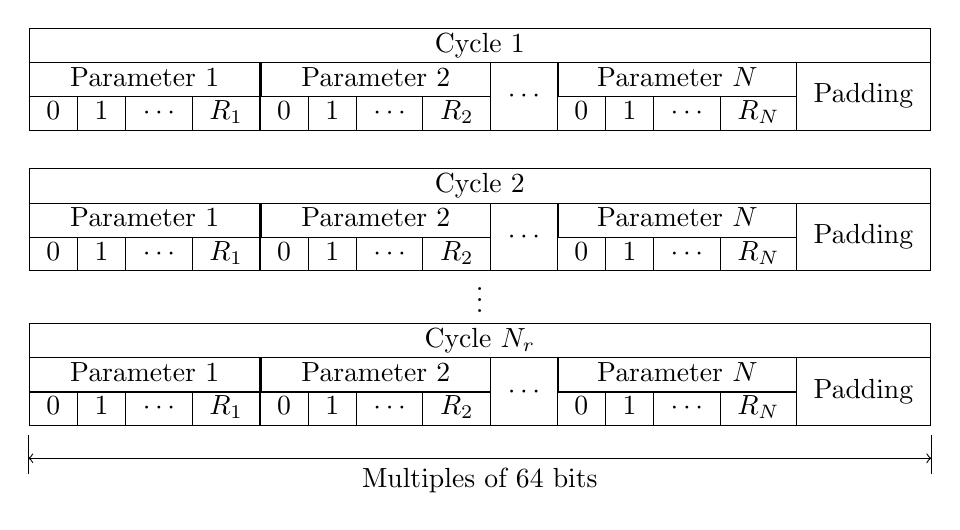
\begin{tikzpicture}
	\node (table) [inner sep=0pt] {
		\begin{tabular}{@{}|c|c|c|c|c|c|c|c|c|c|c|c|c|c|@{}}
			\hline
				\multicolumn{14}{|c|}{Cycle \(1\)} \\
			\hline
				\multicolumn{4}{|c|}{Parameter \(1\)} &
				\multicolumn{4}{|c|}{Parameter \(2\)} &
				\multirow{2}{*}{\(\cdots\)} &
				\multicolumn{4}{|c|}{Parameter \(N\)} &
				\multirow{2}{*}{Padding} \\
			\cline{1-8}
			\cline{10-13}
				0 & 1 & \(\cdots\) & \(R_1\) &
				0 & 1 & \(\cdots\) & \(R_2\) & &
				0 & 1 & \(\cdots\) & \(R_N\) & \\
			\hline
			\multicolumn{8}{c}{\raisebox{1em}{}} \\
			\hline
				\multicolumn{14}{|c|}{Cycle \(2\)} \\
			\hline
				\multicolumn{4}{|c|}{Parameter \(1\)} &
				\multicolumn{4}{|c|}{Parameter \(2\)} &
				\multirow{2}{*}{\(\cdots\)} &
				\multicolumn{4}{|c|}{Parameter \(N\)} &
				\multirow{2}{*}{Padding} \\
			\cline{1-8}
			\cline{10-13}
				0 & 1 & \(\cdots\) & \(R_1\) &
				0 & 1 & \(\cdots\) & \(R_2\) & &
				0 & 1 & \(\cdots\) & \(R_N\) & \\
			\hline
			\multicolumn{14}{c}{\(\vdots\)} \\
			\hline
				\multicolumn{14}{|c|}{Cycle \(N_r\)} \\
			\hline
				\multicolumn{4}{|c|}{Parameter \(1\)} &
				\multicolumn{4}{|c|}{Parameter \(2\)} &
				\multirow{2}{*}{\(\cdots\)} &
				\multicolumn{4}{|c|}{Parameter \(N\)} &
				\multirow{2}{*}{Padding} \\
			\cline{1-8}
			\cline{10-13}
				0 & 1 & \(\cdots\) & \(R_1\) &
				0 & 1 & \(\cdots\) & \(R_2\) & &
				0 & 1 & \(\cdots\) & \(R_N\) & \\
			\hline
		\end{tabular}};
		\foreach \i/\corner in {1/south west, 2/south east}
			\draw (table.\corner) ++(down:3pt) -- ++(down:0.3cm)
			      coordinate (p\i) -- ++(down:0.2cm);
		\draw [<->] (p1) -- (p2)
		      node [midway,anchor=north] {Multiples of 64 bits};
	\end{tikzpicture}
	\caption{Data organization.}
	\label{Fig.DataOrganization}
\end{figure}

\section{Implementation Notes}

\subsection{Decoding the header}

The following snippet of C~code may be used to decode the 6-bit header data.

\begin{lstlisting}[language=C]
void decode(uint8_t *in_buffer, char *out_buffer, size_t length)
{
	uint32_t buf[3];
	for (j = 0, i = 0; i < length; i += 12 /* 3*32/8 */, j += 16) {
		buf[0] = (((uint32_t) in_buffer[i+ 0]) << 24) |
		         (((uint32_t) in_buffer[i+ 1]) << 16) |
		         (((uint32_t) in_buffer[i+ 2]) <<  8) |
		         (((uint32_t) in_buffer[i+ 3]) <<  0);
		buf[1] = (((uint32_t) in_buffer[i+ 4]) << 24) |
		         (((uint32_t) in_buffer[i+ 5]) << 16) |
		         (((uint32_t) in_buffer[i+ 6]) <<  8) |
		         (((uint32_t) in_buffer[i+ 7]) <<  0);
		buf[2] = (((uint32_t) in_buffer[i+ 8]) << 24) |
		         (((uint32_t) in_buffer[i+ 9]) << 16) |
		         (((uint32_t) in_buffer[i+10]) <<  8) |
		         (((uint32_t) in_buffer[i+11]) <<  0);
		out_buffer[j+15] = buf[2] & 0x3F; buf[2] >>= 6;
		out_buffer[j+14] = buf[2] & 0x3F; buf[2] >>= 6;
		out_buffer[j+13] = buf[2] & 0x3F; buf[2] >>= 6;
		out_buffer[j+12] = buf[2] & 0x3F; buf[2] >>= 6;
		out_buffer[j+11] = buf[2] & 0x3F; buf[2] >>= 6;
		out_buffer[j+10] = (buf[2] & 0x3) | ((buf[1] & 0xF) << 2); buf[1] >>= 4;
		out_buffer[j+ 9] = buf[1] & 0x3F; buf[1] >>= 6;
		out_buffer[j+ 8] = buf[1] & 0x3F; buf[1] >>= 6;
		out_buffer[j+ 7] = buf[1] & 0x3F; buf[1] >>= 6;
		out_buffer[j+ 6] = buf[1] & 0x3F; buf[1] >>= 6;
		out_buffer[j+ 5] = (buf[1] & 0xF) | ((buf[0] & 0x3) << 4); buf[0] >>= 2;
		out_buffer[j+ 4] = buf[0] & 0x3F; buf[0] >>= 6;
		out_buffer[j+ 3] = buf[0] & 0x3F; buf[0] >>= 6;
		out_buffer[j+ 2] = buf[0] & 0x3F; buf[0] >>= 6;
		out_buffer[j+ 1] = buf[0] & 0x3F; buf[0] >>= 6;
		out_buffer[j+ 0] = buf[0] & 0x3F; buf[0] >>= 6;
	}
}
\end{lstlisting}


\subsection{Ceiling of division}

It is useful to define a macro to round up integer division (as this operation is required to compute the data offset and stride) such as the following:

\begin{lstlisting}[language=c]
#define DIV_CEIL(n,d) (((n)-1)/(d)+1)
\end{lstlisting}

\section{Using the converter}

The syntax of the converter is straightforward: one specifies the path to the input file, and a path to the desired output file.

\begin{lstlisting}[language=]
$ genpro2nc INFILE OUTFILE
\end{lstlisting}

For example,

\begin{lstlisting}[language=]
$ genpro2nc -b -e bin G50222C
$ genpro2nc G50222C.bin G50222C.nc
\end{lstlisting}

\subsection{Output}

\texttt{genpro2nc} generates a dimension for every variable in the file, named in the form \texttt{\textit{VARIABLE}\_LENGTH}, where \texttt{\textit{VARIABLE}} is the name of the variable. There are two global attributes:
\begin{itemize}
	\item \texttt{CYCLE\_TIME} -- the fundamental sampling period. Sample rates
	      for individual parameters are expressed as multiples of the sampling
	      frequency corresponding to this period.
	\item \texttt{DESCRIPTION} -- the description text found in the input
	      GENPRO-1 file.
\end{itemize}

Every variable has three attributes:
\begin{itemize}
	\item \texttt{DESCRIPTION} -- a human readable description of the variable,
	\item \texttt{UNITS} -- the units of the variable, and
	\item \texttt{SAMPLE\_RATE} -- the sampling frequency for this parameter in multiples of the cycle frequency.
\end{itemize}

\end{document}
